\documentclass[answers]{exam}

\usepackage[dvipsnames]{xcolor}
\usepackage{amsmath}
\usepackage{amsfonts}
\usepackage{amsthm}
\usepackage{microtype}
\usepackage{siunitx}
\DeclareSIUnit\year{yr}
\usepackage{pgfplots}
\usepackage{graphicx}
\usepackage{sidecap}
\sidecaptionvpos{figure}{c}
\usepackage{float}
\usepackage{gensymb}
\usepackage{tkz-euclide}
\usetkzobj{all}
\usepackage{commath}

\newtheorem*{thm}{Theorem}

% russian integral
\usepackage{scalerel}
\DeclareMathOperator*{\rint}{\scalerel*{\rotatebox{17}{$\!\int\!$}}{\int}}

% \qformat{Question \thequestion: \thequestiontitle\hfill}

\begin{document}

\section*{NCEA Level 3 Trigonometry (exercise set)\\1. The Pythagorean Theorem}
\paragraph{Goal} To familiarise ourselves with some of the tools of plane geometry
that we will be utilising this year.

\paragraph{A gentle reminder} My problem sets are intended to be difficult. Thus one should not expect to be able
to write down complete solutions immediately (or even within the week allotted). \emph{This is not a reflection of
your mathematical ability.} Even the best students should have at least one problem that they simply cannot `get',
and this is by design. (If I end up with a student that does write a set of perfect solutions, then I will simply add
another more difficult problem!) My advice would be to make a number of passes: first read all the questions, draw any
diagrams that have not been supplied, and understand in each case what is being asked. Then attempt each problem,
allowing yourself only five or so minutes on each and moving on if you don't get it. Return every day or so to attack
the problems you have not yet completed; and note the attempts you have made, even if they didn't work. (The problems
are not necessarily in order of difficulty, especially since no such ordering exists anyway.)

\begin{questions}
  \question Let $ O $ be a point, and let $ A $ and $ B $ be points distinct from $ O $ (but $ A $ is allowed to be the same point as $ B $).
            Draw the circle of radius 1 centred at $ O $, and let $ \theta $ be the \textbf{anti-clockwise} length\footnote{I will \textbf{always}
            take angles to be in the anti-clockwise direction.} of the circumference of the circle that is cut off by the rays $ \vec{OA} $ and
            $ \vec{OB} $. Then $ \theta $ is said to be the measure of the angle between $ OA $ and $ OB $ (in radians).
            \begin{center}
              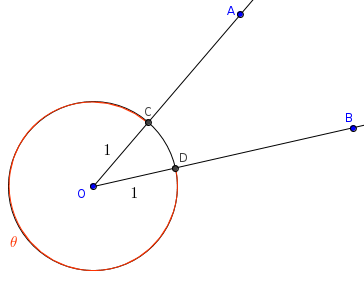
\includegraphics[width=0.3\textwidth]{exercises-1-3}
            \end{center}
            Define the number $ \pi $ to be the measure of a right angle (i.e. one quarter of the unit circle).
    \begin{parts}
      \part Show that if an angle has measure $ \delta $ in degrees, then it has measure $ \frac{\pi\delta}{180} $.
      \part Show that if an angle $ \theta $ is cut through a circle of radius $ r $, then the area of the sector formed between
            the two rays of the angle is $ (\theta r^2)/2 $ and the arc length cut off by the angle is $ \theta r $. [You may
            take for granted that the area of a circle is $ \pi r^2 $ and the length of the circumference is $ 2\pi r $. It is not
            worth being too formal here.]
    \end{parts}
  \question Prove \emph{Thale's theorem}: if $ AB $ is the diameter of a circle, and if $ C $ is any other point on the circle, then
            $ ABC $ is a right triangle with the right angle at $ C $. I can think of three ways right now; try all three:
    \begin{parts}
      \part Use the inscribed angle theorem.
      \part Draw in the angles and push them around (in the same way we proved the inscribed angle theorem).
      \part I'm not telling, try to find another way yourself without getting your hands dirty dealing with angles!
    \end{parts}
  \question Let $ ABDE $ be a square. Pick a point $ C $ inside the square such that the triangle $ CDE $ is isosceles,
            with angles at $ D $ and $ E $ that measure $ \ang{15} = \pi/12 $. What kind of triangle is $ ABC $? (Hint:
            draw another point $ F $ in the square such that $ FBD $ is congruent to $ CED $; what can you say about
            the triangle $ DCF $?)
  \vfill
  \begin{flushright} (cont'd)\end{flushright}
  \clearpage
  \question Recall that a \emph{trapezoid} is a quadrilateral with two opposite sides parallel. For example, in the following
            diagram $ ABCD $ is a trapezoid with parallel sides $ AB $ and $ CD $.

            \begin{center}
              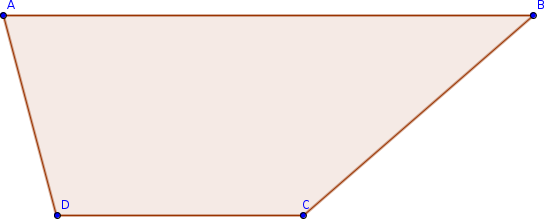
\includegraphics[width=0.3\textwidth]{exercises-1-1}
            \end{center}

            Suppose $ ABCD $ is a trapezoid, with parallel sides $ AB $ and $ CD $; suppose that $ \abs{AB} = a $ and $ \abs{CD} = b $,
            and suppose that the distance between the two parallel sides is $ h $ (the height). Show that $ \mathcal{A}(ABCD) = h\frac{a + b}{2} $.
  \question We have already seen several proofs of the Pythagorean theorem; here is another. This proof is due to a former president
            of the United States of America (James A. Garfield), and is usually accompanied by the observation that ``mathematical ability, while likely a
            hinderance, is thus not a complete disqualification from American politics''.

            Suppose a right triangle $ ABC $ has leg lengths $ a $ and $ b $ and hypotenuse length $ c $. Consider the following figure:

            \begin{center}
              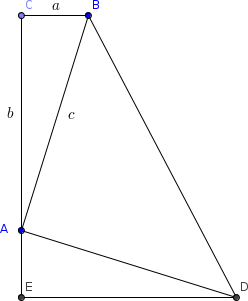
\includegraphics[width=0.3\textwidth]{exercises-1-2}
            \end{center}

            The triangle $ ADE $ is congruent to (has the same lengths and angles as) $ ABC $, so $ \abs{AE} = a $ and $ \abs{ED} = b $.
    \begin{parts}
      \part Show that the angle $ DAB $ is a right angle.
      \part Calculate the area of the trapezoid $ BCED $ in two ways: using the formula from question (4), and by adding
            the areas of the three right triangles $ ABC $, $ ADE $, and $ ABD $.
      \part Deduce that $ a^2 + b^2 = c^2 $.
    \end{parts}
\end{questions}

\paragraph{Additional reading} Coxeter, sections 1.1 to 1.3 inclusive.

\end{document}
